
\documentclass[letterpaper, reqno,11pt]{article}
\usepackage[margin=1.0in]{geometry}
\usepackage{color,latexsym,amsmath,amssymb}
\usepackage{fancyhdr}
\usepackage{amsthm}
\usepackage{mathtools}
\usepackage{tikz}
\usepackage{float}
\usepackage{centernot}
\usepackage{subcaption}
\usepackage{extarrows}
\usetikzlibrary{hobby}
\usetikzlibrary{shapes.multipart}
\usepackage{pgfplots}
\pgfplotsset{compat=1.7}
\usetikzlibrary{arrows.meta}
\usepackage{cancel}
\usetikzlibrary{decorations.markings}
\usetikzlibrary{shapes}
\usetikzlibrary{arrows}
\usepgfplotslibrary{fillbetween}
\usetikzlibrary{patterns}

\newcommand{\RR}{\mathbb{R}}
\newcommand{\CC}{\mathbb{C}}
\newcommand{\ZZ}{\mathbb{Z}}
\newcommand{\QQ}{\mathbb{Q}}
\newcommand{\NN}{\mathbb{N}}
\def\upint{\mathchoice%
  {\mkern13mu\overline{\vphantom{\intop}\mkern7mu}\mkern-20mu}%
  {\mkern7mu\overline{\vphantom{\intop}\mkern7mu}\mkern-14mu}%
  {\mkern7mu\overline{\vphantom{\intop}\mkern7mu}\mkern-14mu}%
  {\mkern7mu\overline{\vphantom{\intop}\mkern7mu}\mkern-14mu}%
  \int}
\def\lowint{\mkern3mu\underline{\vphantom{\intop}\mkern7mu}\mkern-10mu\int}
\DeclareMathOperator{\card}{card}
\DeclareMathOperator{\Binomial}{Binomial}
\DeclareMathOperator{\Span}{span}
\pagestyle{fancy}
\lhead{Math 321 Lecture 26}
\rhead{Yuchong Pan}
\begin{document}
\pagenumbering{arabic}
\title{Math 321 Lecture 26}
\author{Yuchong Pan}
\date{March 11, 2019}
\newtheorem{thm}{Theorem}
\newtheorem{defn}{Definition}
\newtheorem*{remark}{Remark}
\newtheorem{claim}{Claim}
\newtheorem{cor}{Corollary}
\newtheorem{lemma}{Lemma}
\newtheorem{prop}{Proposition}
\newtheorem{fact}{Fact}
\maketitle
%

\section{Dirichlet Kernel}

Recall:
\[ D_N(x) = \frac{\sin\left(\left(N + \frac{1}{2}\right) x\right)}{2 \sin\left(\frac{x}{2}\right)} = \sum_{k = -N}^N e^{ikx}. \]

\begin{claim}
  \normalfont There exists a constant $c_1 > 0$ such that for all $N \geq 1$,
  \[ \lVert D_N \rVert_1 = \frac{1}{2\pi} \int_{-\pi}^\pi |D_N(x)| dx \geq c_1 \log N. \]
\end{claim}

\begin{proof}
  \[ \lVert D_N \rVert_1 = \frac{1}{4\pi} \int_{-\pi}^\pi \frac{\left|\sin\left(\left(N + \frac{1}{2}\right) x\right)\right|}{\left|\sin\left(\frac{x}{2}\right)\right|} dx. \]

  \noindent {\bf Facts:}
  \begin{enumerate}
  \item \label{enum:1} There exists $c > 0$ such that for $x \in [-\pi, \pi]$, $c^{-1} \leq \frac{\left|\sin\left(\frac{x}{2}\right)\right|}{|x|} \leq c$ ($c = 100$ will do).
  \item \label{enum:2} ~

    \begin{figure}[H]
      \centering
      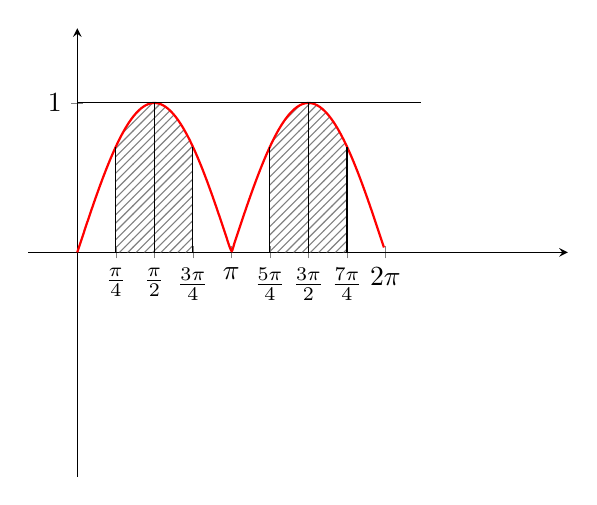
\begin{tikzpicture}
        \begin{axis}[
            xmin=-1,
            xmax=10,
            ymin=-1.5,
            ymax=1.5,
            xtick={0.785, 1.57, 2.355, 3.14, 3.927, 4.712, 5.498, 6.28},
            xticklabels={$\frac{\pi}{4}$, $\frac{\pi}{2}$, $\frac{3\pi}{4}$, $\pi$, $\frac{5\pi}{4}$, $\frac{3\pi}{2}$, $\frac{7\pi}{4}$, $2\pi$},
            ytick={1},
            yticklabels={$1$},
            axis x line=center,
            axis y line=center,
          ]
          \addplot[name path=abssin, thick, red, samples at={0, 0.05, ..., 6.30}, smooth](x,{abs(sin(x/pi*180))});
          \draw (axis cs:pi/4, 0) -- (axis cs:pi/4, {abs(sin(180/4))});
          \draw (axis cs:pi/2, 0) -- (axis cs:pi/2, {abs(sin(180/2))});
          \draw (axis cs:3/4*pi, 0) -- (axis cs:3/4*pi, {abs(sin(3/4*180))});
          \draw (axis cs:5/4*pi, 0) -- (axis cs:5/4*pi, {abs(sin(5/4*180))});
          \draw (axis cs:3/2*pi, 0) -- (axis cs:3/2*pi, {abs(sin(3/2*180))});
          \draw (axis cs:7/4*pi, 0) -- (axis cs:7/4*pi, {abs(sin(7/4*180))});
          \addplot[name path=zero, draw=none, domain={0:10}] {0};
          \addplot[pattern=north east lines, pattern color=gray] fill between[of=abssin and zero, soft clip={domain=pi/4:3/4*pi}];
          \addplot[pattern=north east lines, pattern color=gray] fill between[of=abssin and zero, soft clip={domain=5/4*pi:7/4*pi}];
          \draw (axis cs: 0, 1) -- (axis cs: 7, 1);
        \end{axis}
      \end{tikzpicture}
    \end{figure}

    Since $|\sin t| \geq \frac{1}{\sqrt 2}$ for $t \in (2k + 1) \frac{\pi}{2} + \left[-\frac{\pi}{4}, \frac{\pi}{4}\right], k \in \ZZ$, we conclude that
    \[ \left|\sin\left(\left(N + \frac{1}{2}\right) x\right)\right| \geq \frac{1}{\sqrt 2} \text{ whenever } \left|\left(N + \frac{1}{2}\right) x - (2k + 1) \frac{\pi}{2}\right| < \frac{\pi}{4} \text{ for some $k \in \ZZ$}. \]
    Note that
    \begin{align*}
      & \left|\left(N + \frac{1}{2}\right) x - (2k + 1) \frac{\pi}{2}\right| < \frac{\pi}{4} \\
      \Leftrightarrow ~ & \left|x - \frac{2k + 1}{N + \frac{1}{2}} \cdot \frac{\pi}{2}\right| < \frac{\pi}{4\left(N + \frac{1}{2}\right)} \\
      \Leftrightarrow ~ & \underbrace{\boxed{\left|x - \frac{2k + 1}{2N + 1} \cdot \pi\right| < \frac{\pi}{4N + 2}}}_\text{call this interval $I_k$}.
    \end{align*}

    \begin{figure}[H]
      \centering
      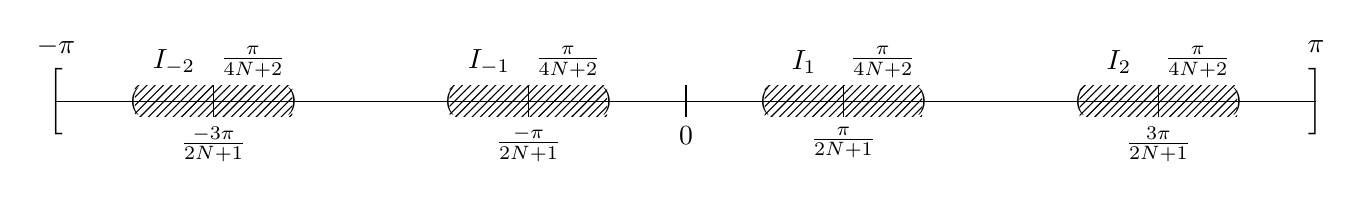
\begin{tikzpicture}
        \draw (-8, 0) -- (8, 0);
        \draw (0, 0.2) -- (0, -0.2) node[below] {$0$};
        \draw (2, 0.2) -- (2, -0.2) node[below] {$\frac{\pi}{2N + 1}$};
        \draw (6, 0.2) -- (6, -0.2) node[below] {$\frac{3\pi}{2N + 1}$};
        \draw (-2, 0.2) -- (-2, -0.2) node[below] {$\frac{-\pi}{2N + 1}$};
        \draw (-6, 0.2) -- (-6, -0.2) node[below] {$\frac{-3\pi}{2N + 1}$};
        \node at (1, 0) {$($};
        \node at (3, 0) {$)$};
        \node at (5, 0) {$($};
        \node at (7, 0) {$)$};
        \node at (-3, 0) {$($};
        \node at (-1, 0) {$)$};
        \node at (-7, 0) {$($};
        \node at (-5, 0) {$)$};
        \fill[pattern=north east lines] (1, 0.2) rectangle (3, -0.2);
        \fill[pattern=north east lines] (5, 0.2) rectangle (7, -0.2);
        \fill[pattern=north east lines] (-3, 0.2) rectangle (-1, -0.2);
        \fill[pattern=north east lines] (-7, 0.2) rectangle (-5, -0.2);
        \node at (2.5, 0.5) {$\frac{\pi}{4N + 2}$};
        \node at (6.5, 0.5) {$\frac{\pi}{4N + 2}$};
        \node at (-1.5, 0.5) {$\frac{\pi}{4N + 2}$};
        \node at (-5.5, 0.5) {$\frac{\pi}{4N + 2}$};
        \node at (1.5, 0.5) {$I_1$};
        \node at (5.5, 0.5) {$I_2$};
        \node at (-2.5, 0.5) {$I_{-1}$};
        \node at (-6.5, 0.5) {$I_{-2}$};
        \node at (-8, 0) {$\bigg [$};
          \node at (8, 0) {$\bigg ]$};
        \node at (-8, 0.7) {$-\pi$};
        \node at (8, 0.7) {$\pi$};
      \end{tikzpicture}
    \end{figure}

    Need to ensure that these intervals fall within $[-\pi, \pi]$, so suffices to impose the condition
    \begin{align*}
      -\pi < \frac{2k + 1}{2N + 1} \pi < \pi & \Rightarrow -1 < \frac{2k + 1}{2N + 1} < 1 \\
      & \Rightarrow -2N - 1 < 2k + 1 < 2N + 1 \\
      & \Rightarrow \boxed{-N - 1 < k < N}.
    \end{align*}
  \end{enumerate}
  
  Combine Facts \ref{enum:1} and \ref{enum:2},
  \begin{align*}
    \lVert D_N \rVert_1 &\geq \sum_{k = N}^{N - 1} \int_{I_k} \left|\frac{\sin\left(\left(N + \frac{1}{2}\right) x\right)}{\sin\left(\frac{x}{2}\right)}\right| dx \\
    &\overset{(\ref{enum:2})}{\geq} \frac{1}{\sqrt 2} \sum_{k = -N}^N \int_{I_k} \frac{1}{\left|\sin\left(\frac{x}{2}\right)\right|} dx \\
    &\geq \frac{c^{-1}}{\sqrt 2} \sum_{k = -N}^N \int_{I_k} \frac{dx}{|x|} \\
    &\geq \frac{c^{-1}}{\sqrt 2} \sum_{k = -N}^N \frac{1}{\frac{2k + 1}{2N + 1} \pi + \frac{\pi}{4N + 2}} \cdot \frac{2\pi}{4N + 2} \\
    &\geq c_0 \sum_{k = -N}^N \underbrace{\frac{1}{2k + \frac{3}{2}}}_\text{comparable to the harmonic series} \\
    &\geq c_1' \sum_{k = -N}^{N - 1} \frac{1}{k} \geq c_1 \log N.
  \end{align*}
\end{proof}

\begin{remark}
  \normalfont
  ~
  
  \begin{enumerate}
  \item Note that
    \[ c_1 \log N \leq \lVert D_N \rVert_1 \leq \underbrace{\lVert D_N \rVert_2}_\text{Plancherel: $\sqrt{\substack{\text{sum of squares of the} \\ \text{Fourier coefficients of $D_N$}}} = \sqrt{2N + 1}$}. \]
  \item An example of a function $f \in \mathcal C^{2\pi}$ whose Fourier series does not converge uniformly: In HW 9, Q3 (b), you found $f \in \mathcal C^{2\pi}$ such that
    \begin{equation} \label{eq:*} \tag{*}
      \sup_N |s_N f(0)| = \infty.
    \end{equation}
    If $s_N f \to f$ uniformly on $[-\pi, \pi]$, then $s_N f(0) \xrightarrow{N \to \infty} f(0)$; not possible by \eqref{eq:*}.
  \item Question: What is $\lVert D_N \rVert_\infty$? $\lVert D_N \rVert_\infty = 2N + 1$.
    \[ |D_N(x)| = \frac{\left|\sin\left(\left(N + \frac{1}{2}\right) x\right)\right|}{\left|\sin\left(\frac{x}{2}\right)\right|} = \left|\sum_{k = -N}^N e^{ikx}\right| \underbrace{\leq}_\text{equality when $x = 0$} \sum_{k = -N}^N \underbrace{\left|e^{ikx}\right|}_{= 1} = 2N + 1. \]
  \end{enumerate}
\end{remark}

\section{Convergence of Fourier Series}

\begin{thm}
  \normalfont Suppose $f \in \mathcal C^{2\pi}$ is twice continuously differentiable. Then $s_N f \xrightarrow{N \to \infty} f$ uniformly.
\end{thm}

\begin{proof}
  \begin{align*}
    \widehat f(k) &= \frac{1}{2\pi} \int_{-\pi}^\pi f(x) e^{-ikx} dx \\
    &\overset{\text{IBP}}{=} \frac{1}{2\pi} \left[\cancelto{0}{\left.f(x) \frac{e^{-ikx}}{-ik}\right|_{-\pi}^\pi} - \int_{-\pi}^\pi f'(x) \frac{e^{-ikx}}{-ik} dx\right] \\
    &= \frac{1}{2\pi ik} \int_{-\pi}^\pi f'(x) e^{-ikx} dx \\
    &\overset{\text{IBP}}{=} \frac{1}{2\pi ik} \left[\left.f'(x) \frac{e^{-ikx}}{-ik}\right|_{-\pi}^\pi - \int_{-\pi}^\pi f''(x) \frac{e^{-ikx}}{-ik} dx\right].
  \end{align*}
  \begin{align*}
    &\Rightarrow \left|\widehat f(k)\right| \leq \frac{c}{k^2} \\
    &\xRightarrow{\text{by $M$-test}} \sum_{k \in \ZZ} \widehat f(k) e^{ikx} \text{ converges uniformly to some $g \in \mathcal C^{2\pi}$}.
  \end{align*}
  \begin{align*}
    \text{Plancherel} &\Rightarrow \sum_{k \in \ZZ} \widehat f(k) e^{ikx} \text{ converges in $L^2$ to $f \in \mathcal C^{2\pi}$} \\
    &\Rightarrow \lVert f - g \rVert_2 = 0 \\
    &\Rightarrow f \equiv g \text{ since $f, g \in \mathcal C^{2\pi}$}.
  \end{align*}
\end{proof}

\end{document}
